% Add \usepackage{graphicx}. Paths assume compilation from the repository root.
% Full-width 7.16-inch figures. For an IEEE two-column template use figure*.
\begin{figure}[t]
  \centering
  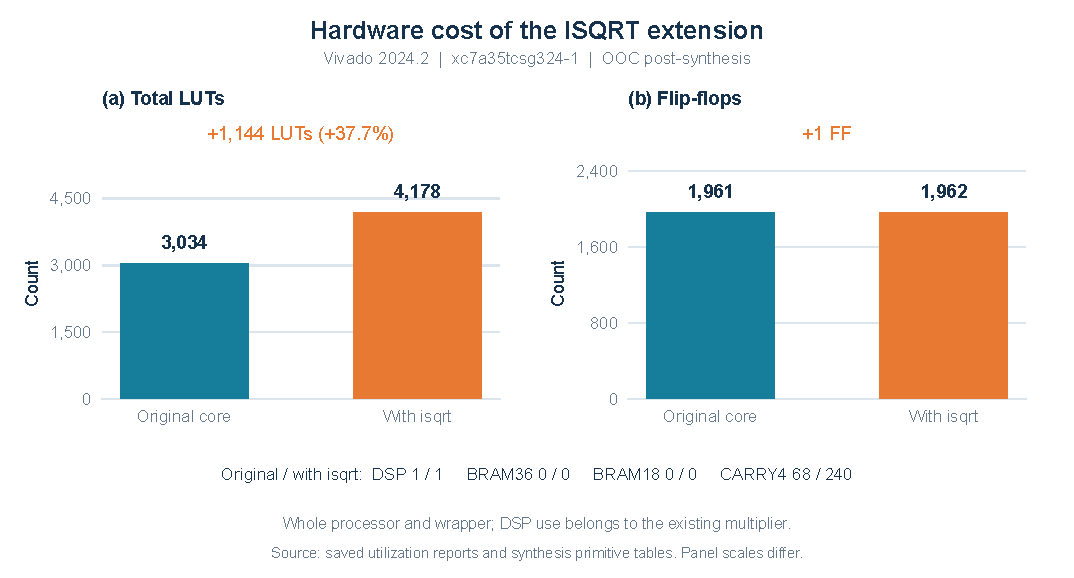
\includegraphics[width=\linewidth]{output/pdf/fig05_fpga_resources.pdf}
  \caption{Whole-design FPGA resource utilization for the original CVE2 and the isqrt extension, parsed from Vivado out-of-context post-synthesis reports. Total LUTs and FFs use the top-level utilization row; CARRY4 counts come from the synthesis primitive table. The paired point plots use circles for the original and diamonds for isqrt. Both designs include the same wrapper and processor configuration. Panel scales differ. The DSP belongs to the existing multiplier; no implemented area is claimed.}
  \label{fig:fig05_fpga_resources}
\end{figure}

\begin{figure}[t]
  \centering
  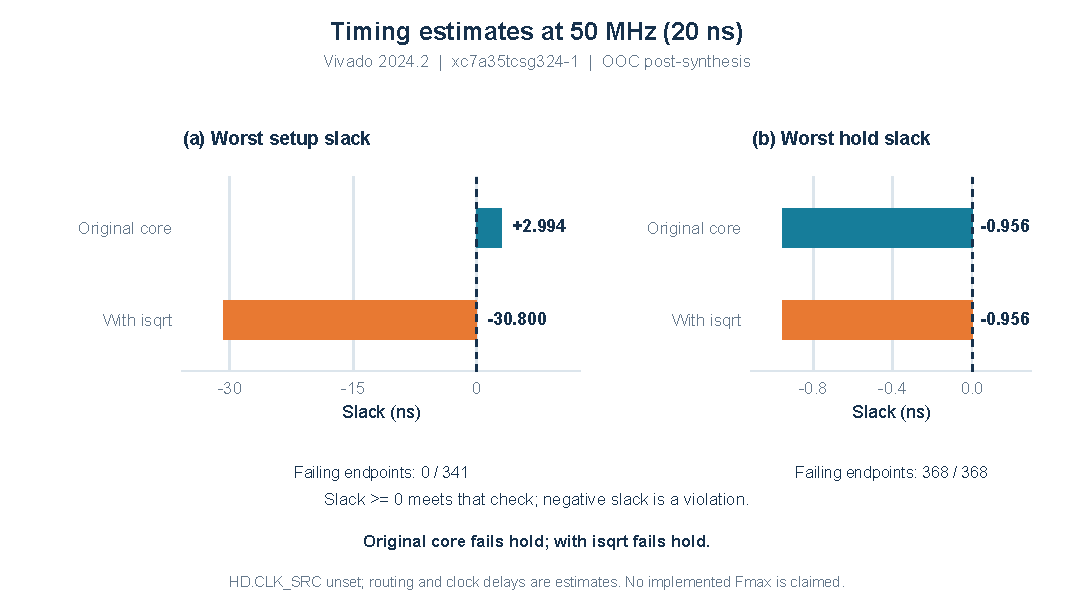
\includegraphics[width=\linewidth]{output/pdf/fig06_fpga_timing.pdf}
  \caption{Heatmap of worst setup, hold and pulse-width slack from the complete design timing summaries for both cores at the same clock target. All colors share one diverging nanosecond scale centered on zero. Each cell also reports failing and total endpoints. Nonnegative slack meets the corresponding check. Original core passes setup; with isqrt fails setup. Original core fails hold; with isqrt fails hold. These are out-of-context post-synthesis estimates with an unset HD.CLK\_SRC clock context. They do not establish routed timing closure or implemented Fmax.}
  \label{fig:fig06_fpga_timing}
\end{figure}

\begin{figure}[t]
  \centering
  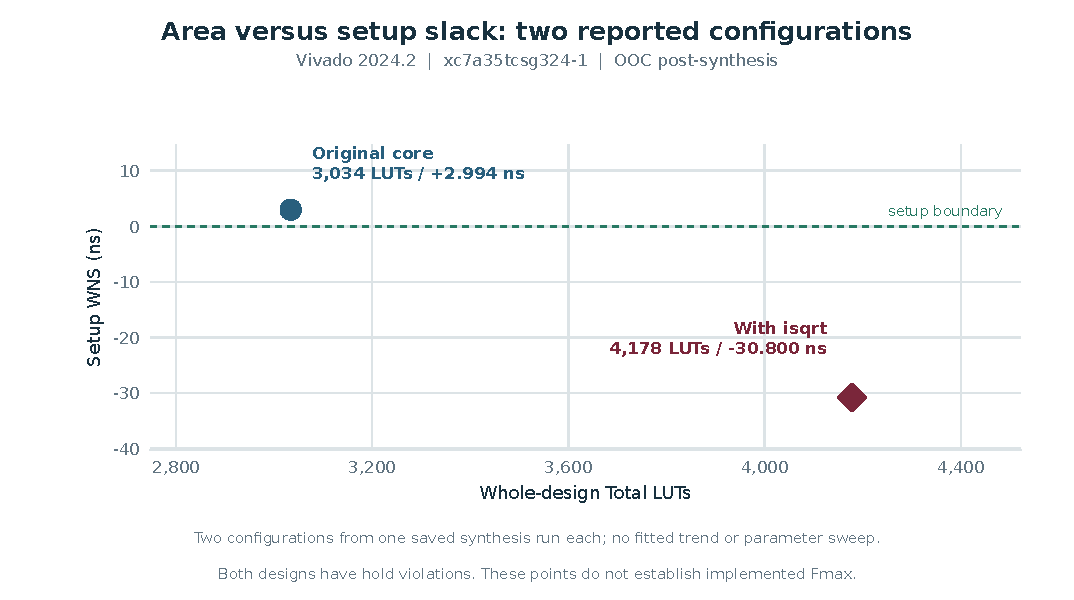
\includegraphics[width=\linewidth]{output/pdf/fig07_fpga_tradeoff.pdf}
  \caption{Scatter plot of whole-design Total LUTs against worst setup slack for the two saved synthesis configurations. Each marker represents one run; there is no parameter sweep, fitted trend or statistical replication. The zero-slack reference concerns setup only. Both designs have hold violations, and routing and clock delays remain estimates.}
  \label{fig:fig07_fpga_tradeoff}
\end{figure}

\begin{figure}[t]
  \centering
  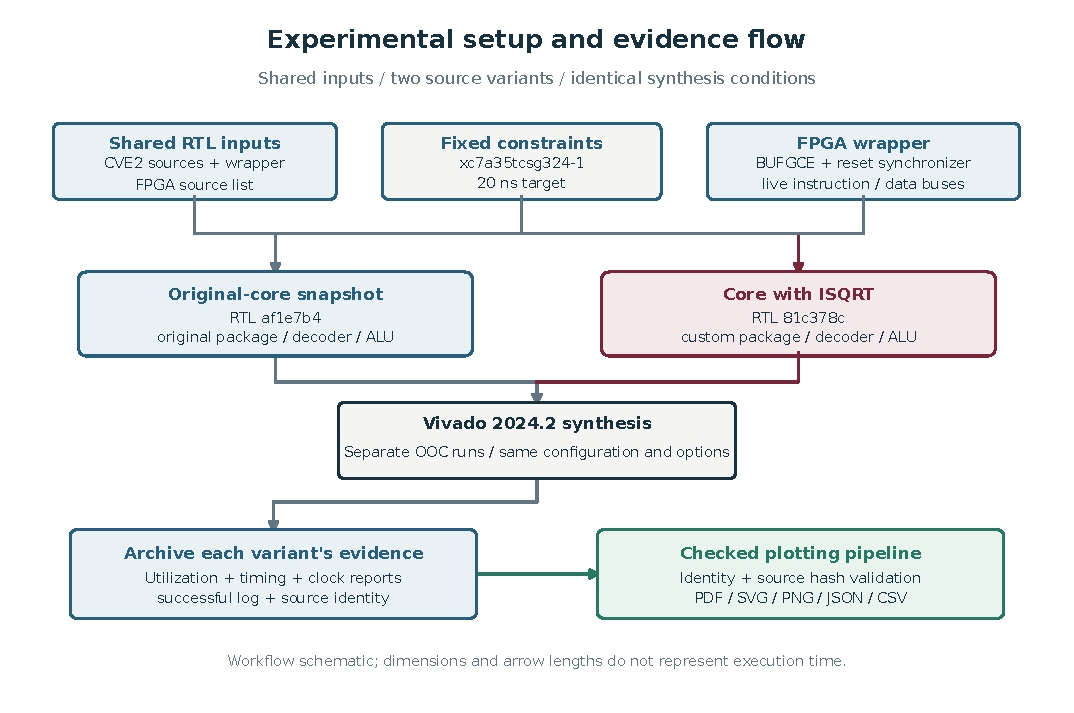
\includegraphics[width=\linewidth]{output/pdf/fig08_experimental_setup.pdf}
  \caption{Schematic of the recorded FPGA experiment and evidence pipeline. The original snapshot and extended core share the wrapper, source list, part, clock constraints, configuration and synthesis options. Reports, successful logs and source identity feed the checked plotting script. This is a workflow illustration, not a measurement of latency or hardware area.}
  \label{fig:fig08_experimental_setup}
\end{figure}
